\chapter{Method and materials}


\section{Study area} % flyttet først etter AMkomm
%mogleg å kjøre ein fin overgang fra intro til study area? Study area valt pga dårlige snøforhold i nyere tid -> vanskelig å gjere spor-tellinger -> denne delen av landet har starta med CT (\cite{Odden2015})


The mean annual temperatures ranges from 2-6 \celsius , precipitation lies between 700-1500mm and growing season length lies between 170 - 190 days (\cite{Moen1999}).
Topography is predominantly flat towards the south, and more rugged and elevated towards the north. The landscape is a mosaic of forest and agricultural areas, divided with a wide network of gravel roads.
The area is situated in the southern boreal and the boreonemoral zones. %Må finne oppdaterte data (frå Norges vassdrags- og energidirektorat, 2019?)
Norway spruce (\textit{Picea abies}) and Scots pine (\textit{Pinus sylvestris}) make up the dominating boreal coniferous forests, with frequent presence of silver birch (\textit{Betula pendula}) and downy birch (\textit{Betula pubescens}), then aspen (\textit{Populous tremula}), alder (\textit{Alnus incana}) and black alder (\textit{Alnus glutinosa}).


%https://klimaservicesenter.no/faces/desktop/article.xhtml?uri=klimaservicesenteret/klimaprofiler/klimaprofil-oslo-og-akershus
%https://klimaservicesenter.no/faces/desktop/article.xhtml?uri=klimaservicesenteret%2Fklimaprofiler%2Fklimaprofil-buskerud  
The study area (59.36-60.45° N, 9.31-11.13° E) extends over much of the southeastern parts of Norway in municipalities Flå, Krødsherad, Sigdal, Ringerike, Modum, Hole, Lier, Øvre Eiker, Asker, Oslo, Enebakk, Indre Østfold, Våler, Råde, Moss, Frogn and Vestby in Oslo and Viken counties. 
The climate has a continental character due to rain shadows of the mountain ridges from the west. 


\section{Study species} %Usikker på om eg skal ha med
%\subsubsection{Rev}  ?

%We also collated information on average body and home range sizes for a subset of species surveyed in the reviewed studies in order to better quantify the functional diversity of wildlife being sampled by CTs and to evaluate the degree to which CT methodologies were tailored to focal species. Burton 2015

The species I'll focus on in this thesis are the species that most frequently was observed \emph{(>50 events)}, excluding farmed animals (e.g. cattle), humans and dogs, and grouped categories of animals (e.g. birds).
%Although decisions on camera placement (height and angle) were made with the aim on photo capturing lynx, I have also included smaller species in the analysis.

That left nine species, namely roe deer (\textit{Capreolus capreolus}), red fox (\textit{Vulpes vulpes}), badger (\textit{Meles meles}), moose (\textit{Alces alces}), red deer (\textit{Cervus elaphus}), red squirrel (\textit{Sqiurus vulgaris}), hare (\textit{Lepus timidus}), European pine marten (\textit{Martes martes}) and lynx. 




\section{Study design} 


The Norwegian Institute of Nature Research (NINA) started with CTs to substitute snow track surveys of lynx family groups, after several years of varying snow season length in south eastern Norway (\cite{Odden2015}). The surveys are integrated in a coordinated Scandinavian science project on lynx, called Scandlynx. % Beddari siterte SCANDLYNX2017  

I was given access to CTs used in the Scandlynx project, and chose 60 sites to get a substantial amount of data, while doing a feasible amount of field work besides my master courses at the university.
For logistical reasons, I chose the sites closest to Oslo which weren't already equipped with white LED flashes. 
Instead, these CTs were equipped with infra-red flashes, and I will refer to them as the \emph{IR CTs}.


The IR CTs had been installed on trees 1-3 m from wildlife, human or tractor paths, 30-160 cm above ground level, and their distance from houses or roads varied to a large extent.
They were set up and handled by people from NINA and, at the sites further from Oslo, by local volunteers. %members of the Norwegian Hunters and Fishers Society (NJFF). 
The installation of the cameras did not follow a strict protocol, nor were their locations chosen randomly. The overall placement was systematic as decided by NINA, then there was a deliberately-biased placement of the CTs put up in areas where the individual handler deemed it most likely to photograph lynx, and hence, based on a combination of site accessibility and expectations of animal occurrence. % slik som (\cite{Burton2015} seier skal formidlast). 


\begin{figure}
    \begin{center}
    	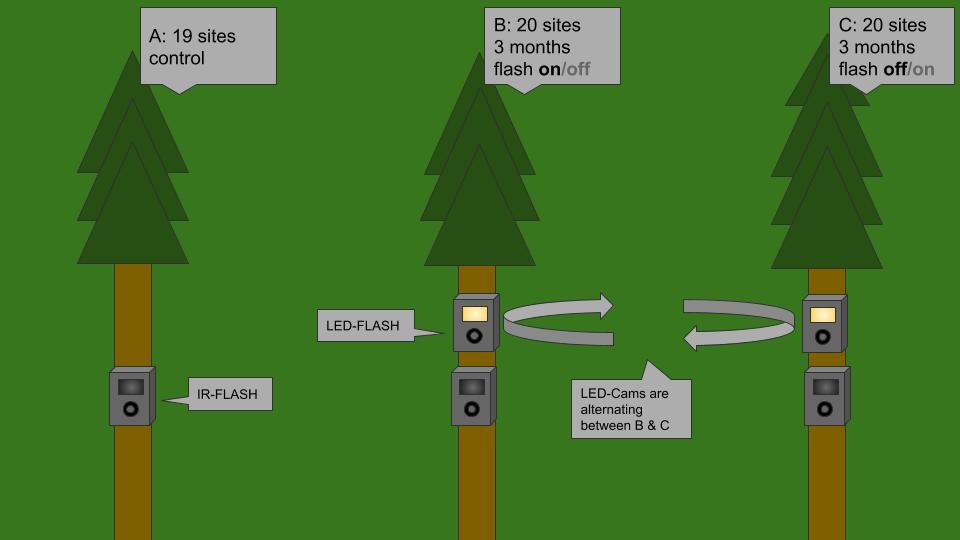
\includegraphics[scale=0.4]{./img/experiment_setup.jpg} %insert figure of groups     
    \end{center}
\caption[Experiment setup]
    	{Experiment setup %\par \small
    	 I chose 60 sites with preinstalled Infrared Camera Traps (IR CTs) for my study, and divided them into three groups, where the first group remained unchanged (control group), and the two other alternated on having additional white LED CTs present (treatment groups). Four sites were removed from the analysis due to large gaps in the data, etc.}
    \label{fig:exp_set}
\end{figure} 


I divided the sites randomly into three groups of 20 sites.
The first group remained unchanged as a control, and the remaining two groups (hereby referred to as the \emph{treatment groups}) were equipped with an additional white LED camera (hereby referred to as the \emph{wLED CTs}) in alternating 3 month-periods, as illustrated in figure\vref{fig:exp_set}.
Periods when an additional wLED CT was present, I will refer to as \emph{wLED periods}.
Periods when the wLED was absent, I will refer to as \emph{IR periods}.
All periods from the control group, I will refer to as \emph{control periods}.
Note that control periods also are periods with only IR CTs present, but they differ from the IR periods in that there never was a white LED present at these sites.


%After approximately three months, I moved the LED CTs to the other treatment group. The periods were marked as LED\_1, LED\_2 for first and second LED period, and IR\_1, IR\_2 for first and second IR period as seen in figure \vref{fig:timeseries}.
I set up all wLED CTs above the IR CTs already in place (installation examples in figure \ref{fig:cam_ex_main}), using an electric drill. 
I used short logs to adjust the angle of the wLED CTs, aligning it to the IR CTs field of view.
Vegetation obstructing the view of any camera was removed at setup, or when noticed during a later visitation (e.g. tall grass during summer).

 
At one site the IR camera had been installed so far above ground level that I chose to position the wLED CT below the IR CT. %Atle fjerna kryssref til bildet

The camera boxes containing the wLED CTs remained at each site untill the end of the survey. Note that the second treatment group had no extra boxes  before the start of their first wLED period in May 2019.   



\begin{figure}
		\begin{subfigure}{.5\textwidth}
		  \centering
		  	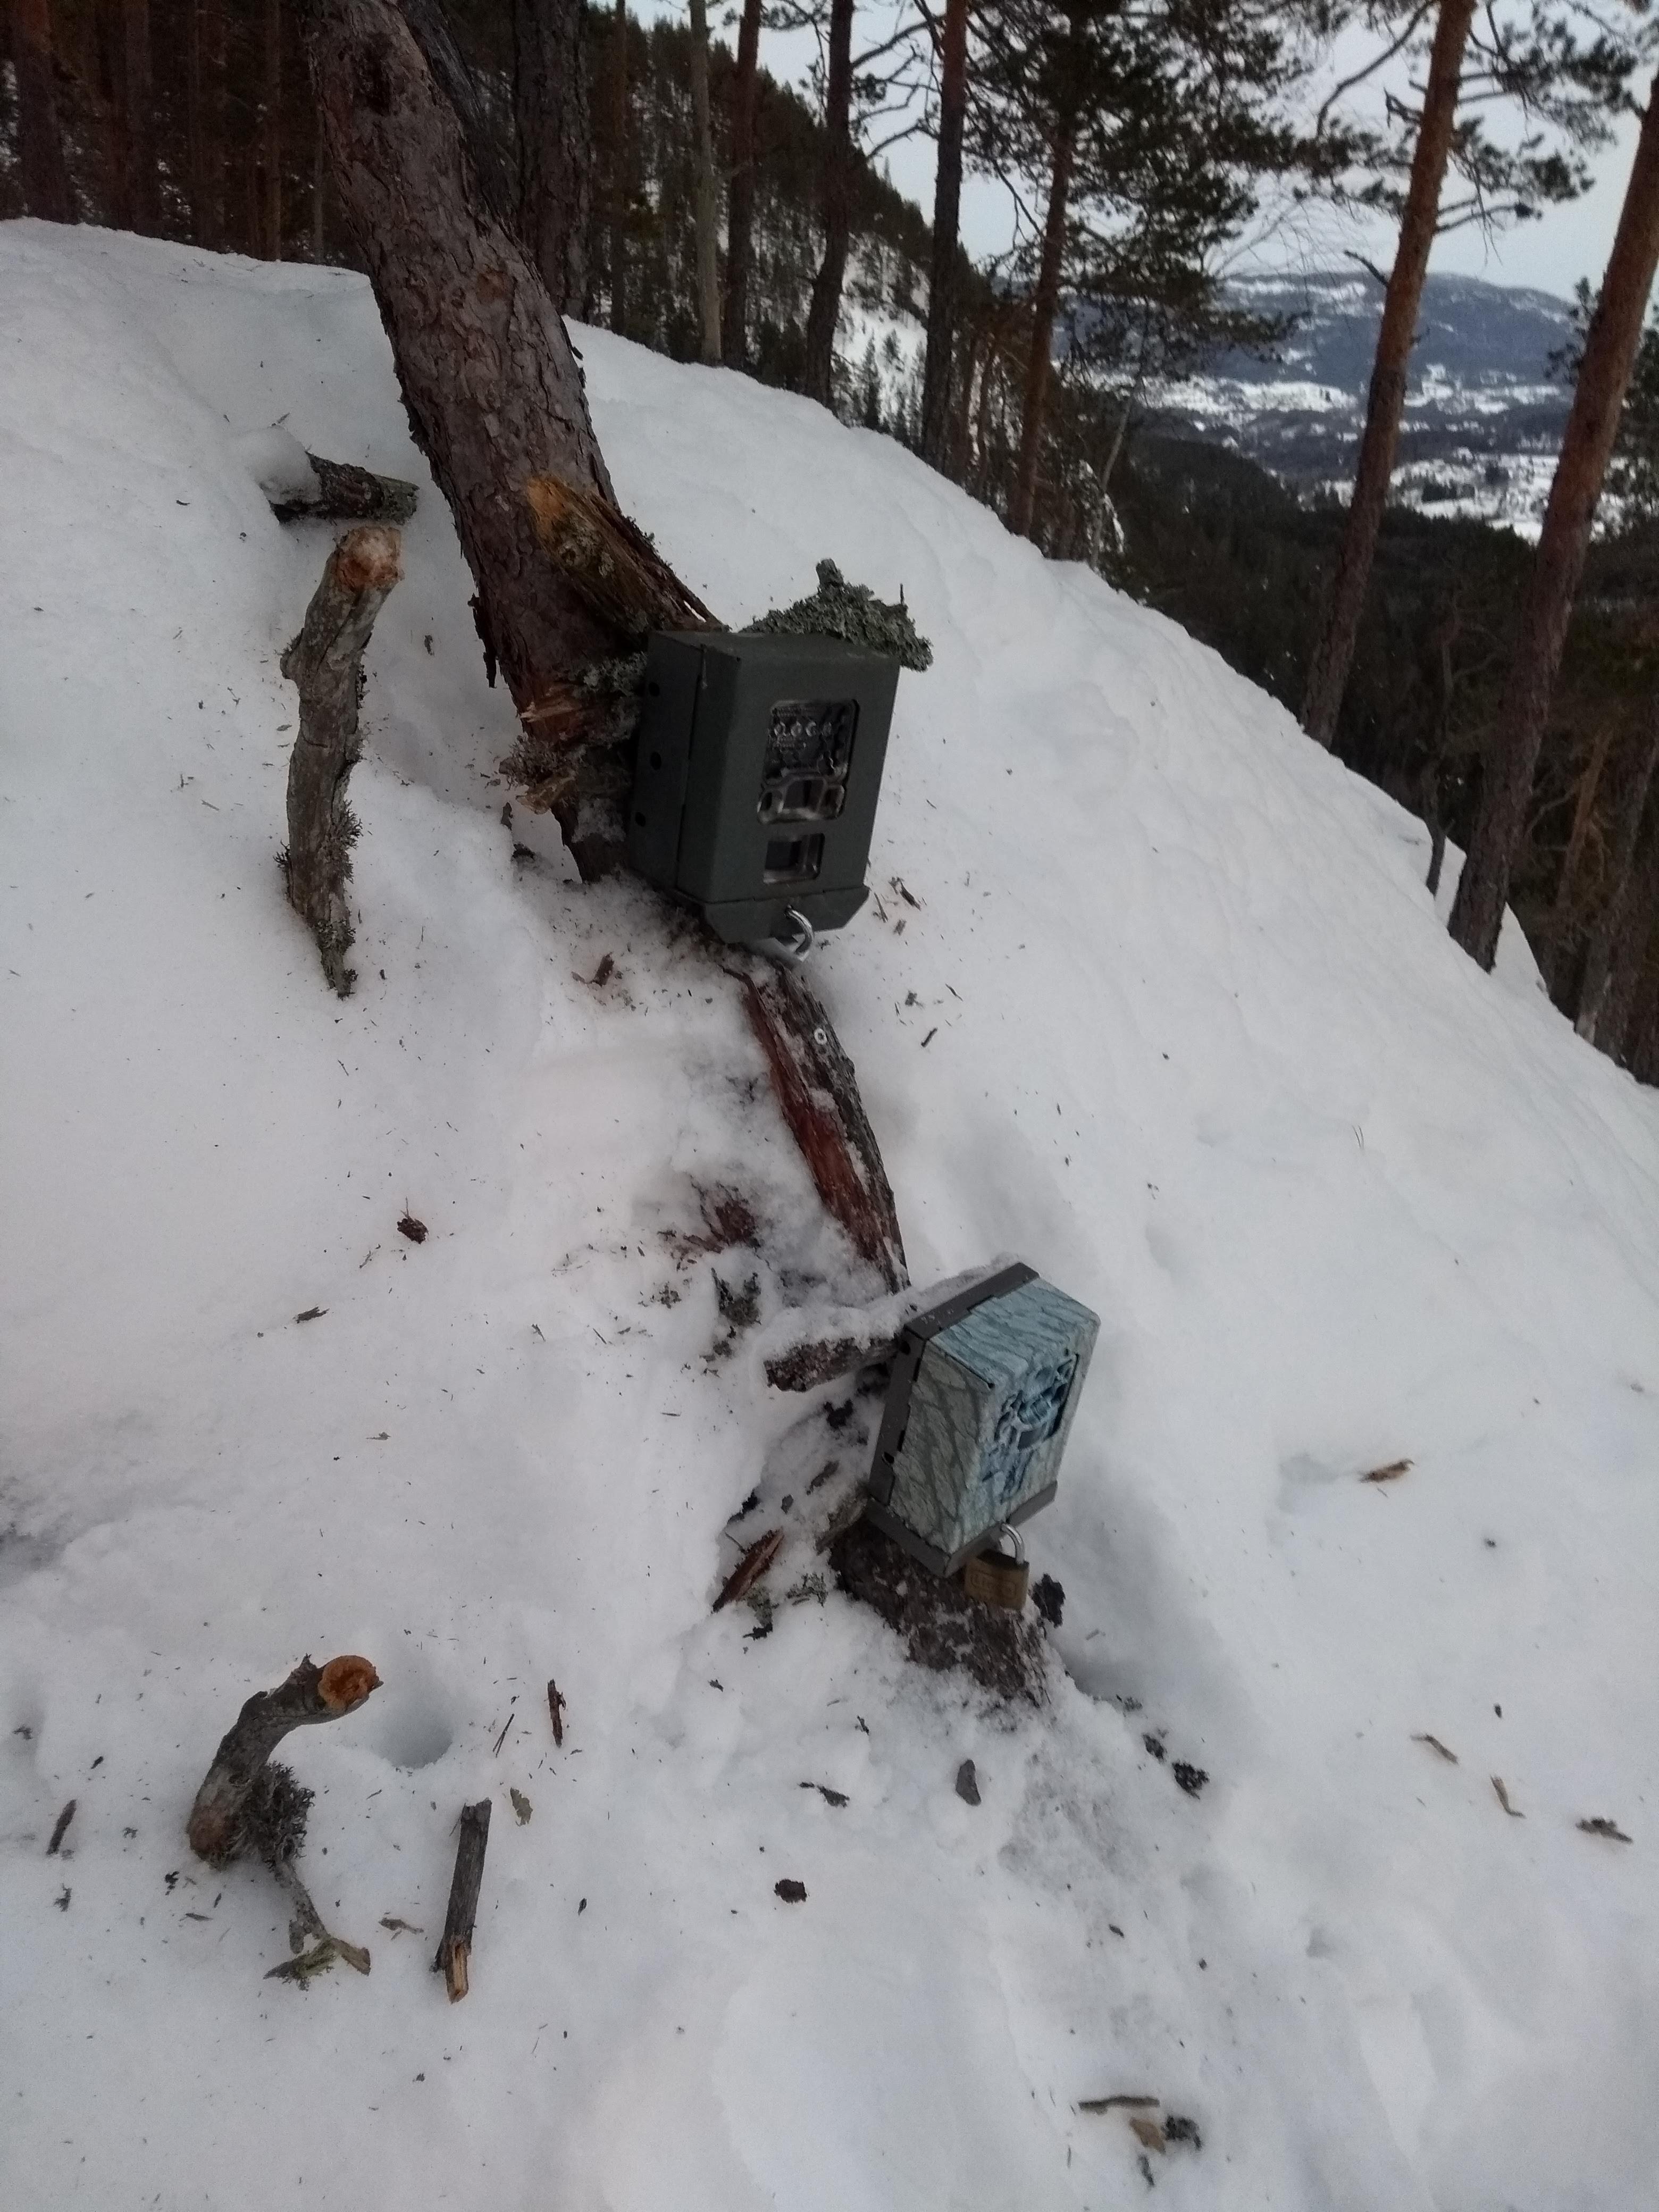
\includegraphics[width=.8\linewidth]{./img/cam_install_example/IMG_20190212_161615169.jpg}
		  \caption{Browning IR installed on fallen tree.}
		  	\label{fig:cam_ex_a}
	\end{subfigure}
		\begin{subfigure}{.5\textwidth}
		  \centering
		  	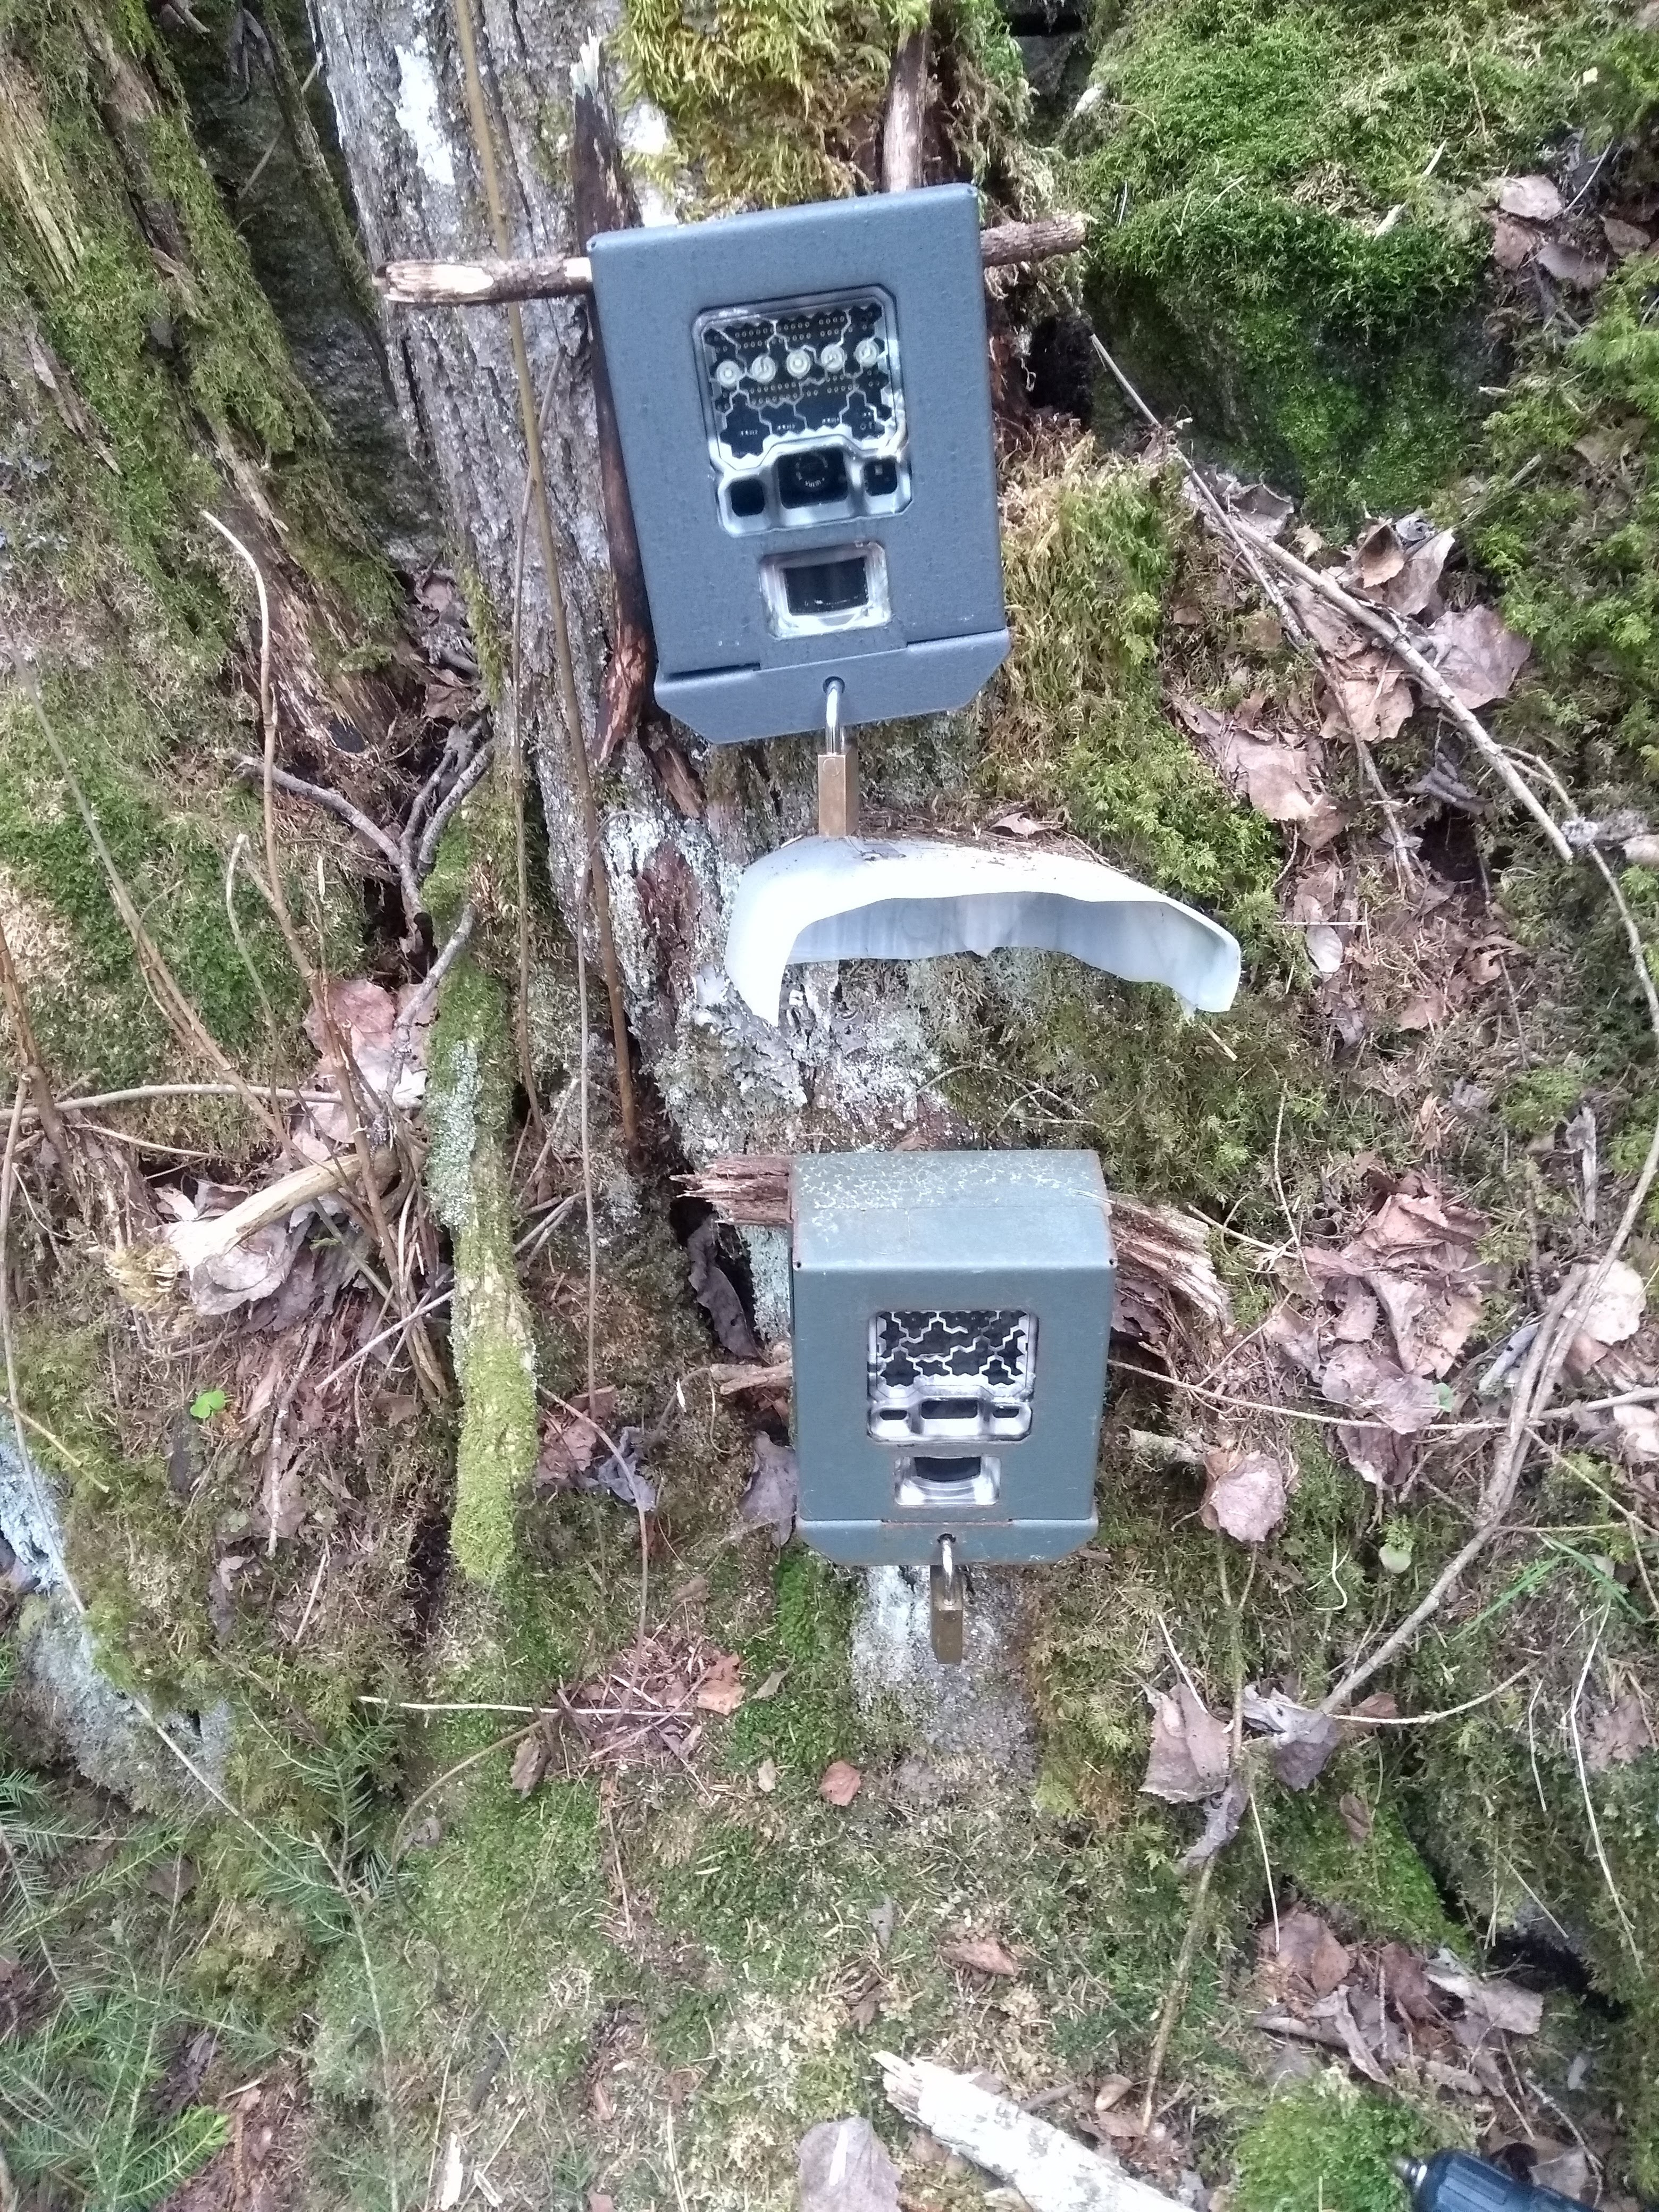
\includegraphics[width=.8\linewidth]{./img/cam_install_example/IMG_20190515_170952923.jpg}
		  \caption{Reconyx IR installed with snow cap.}
		  	\label{fig:cam_ex_b}
	\end{subfigure}
		\begin{subfigure}{.5\textwidth}
		  \centering
		  	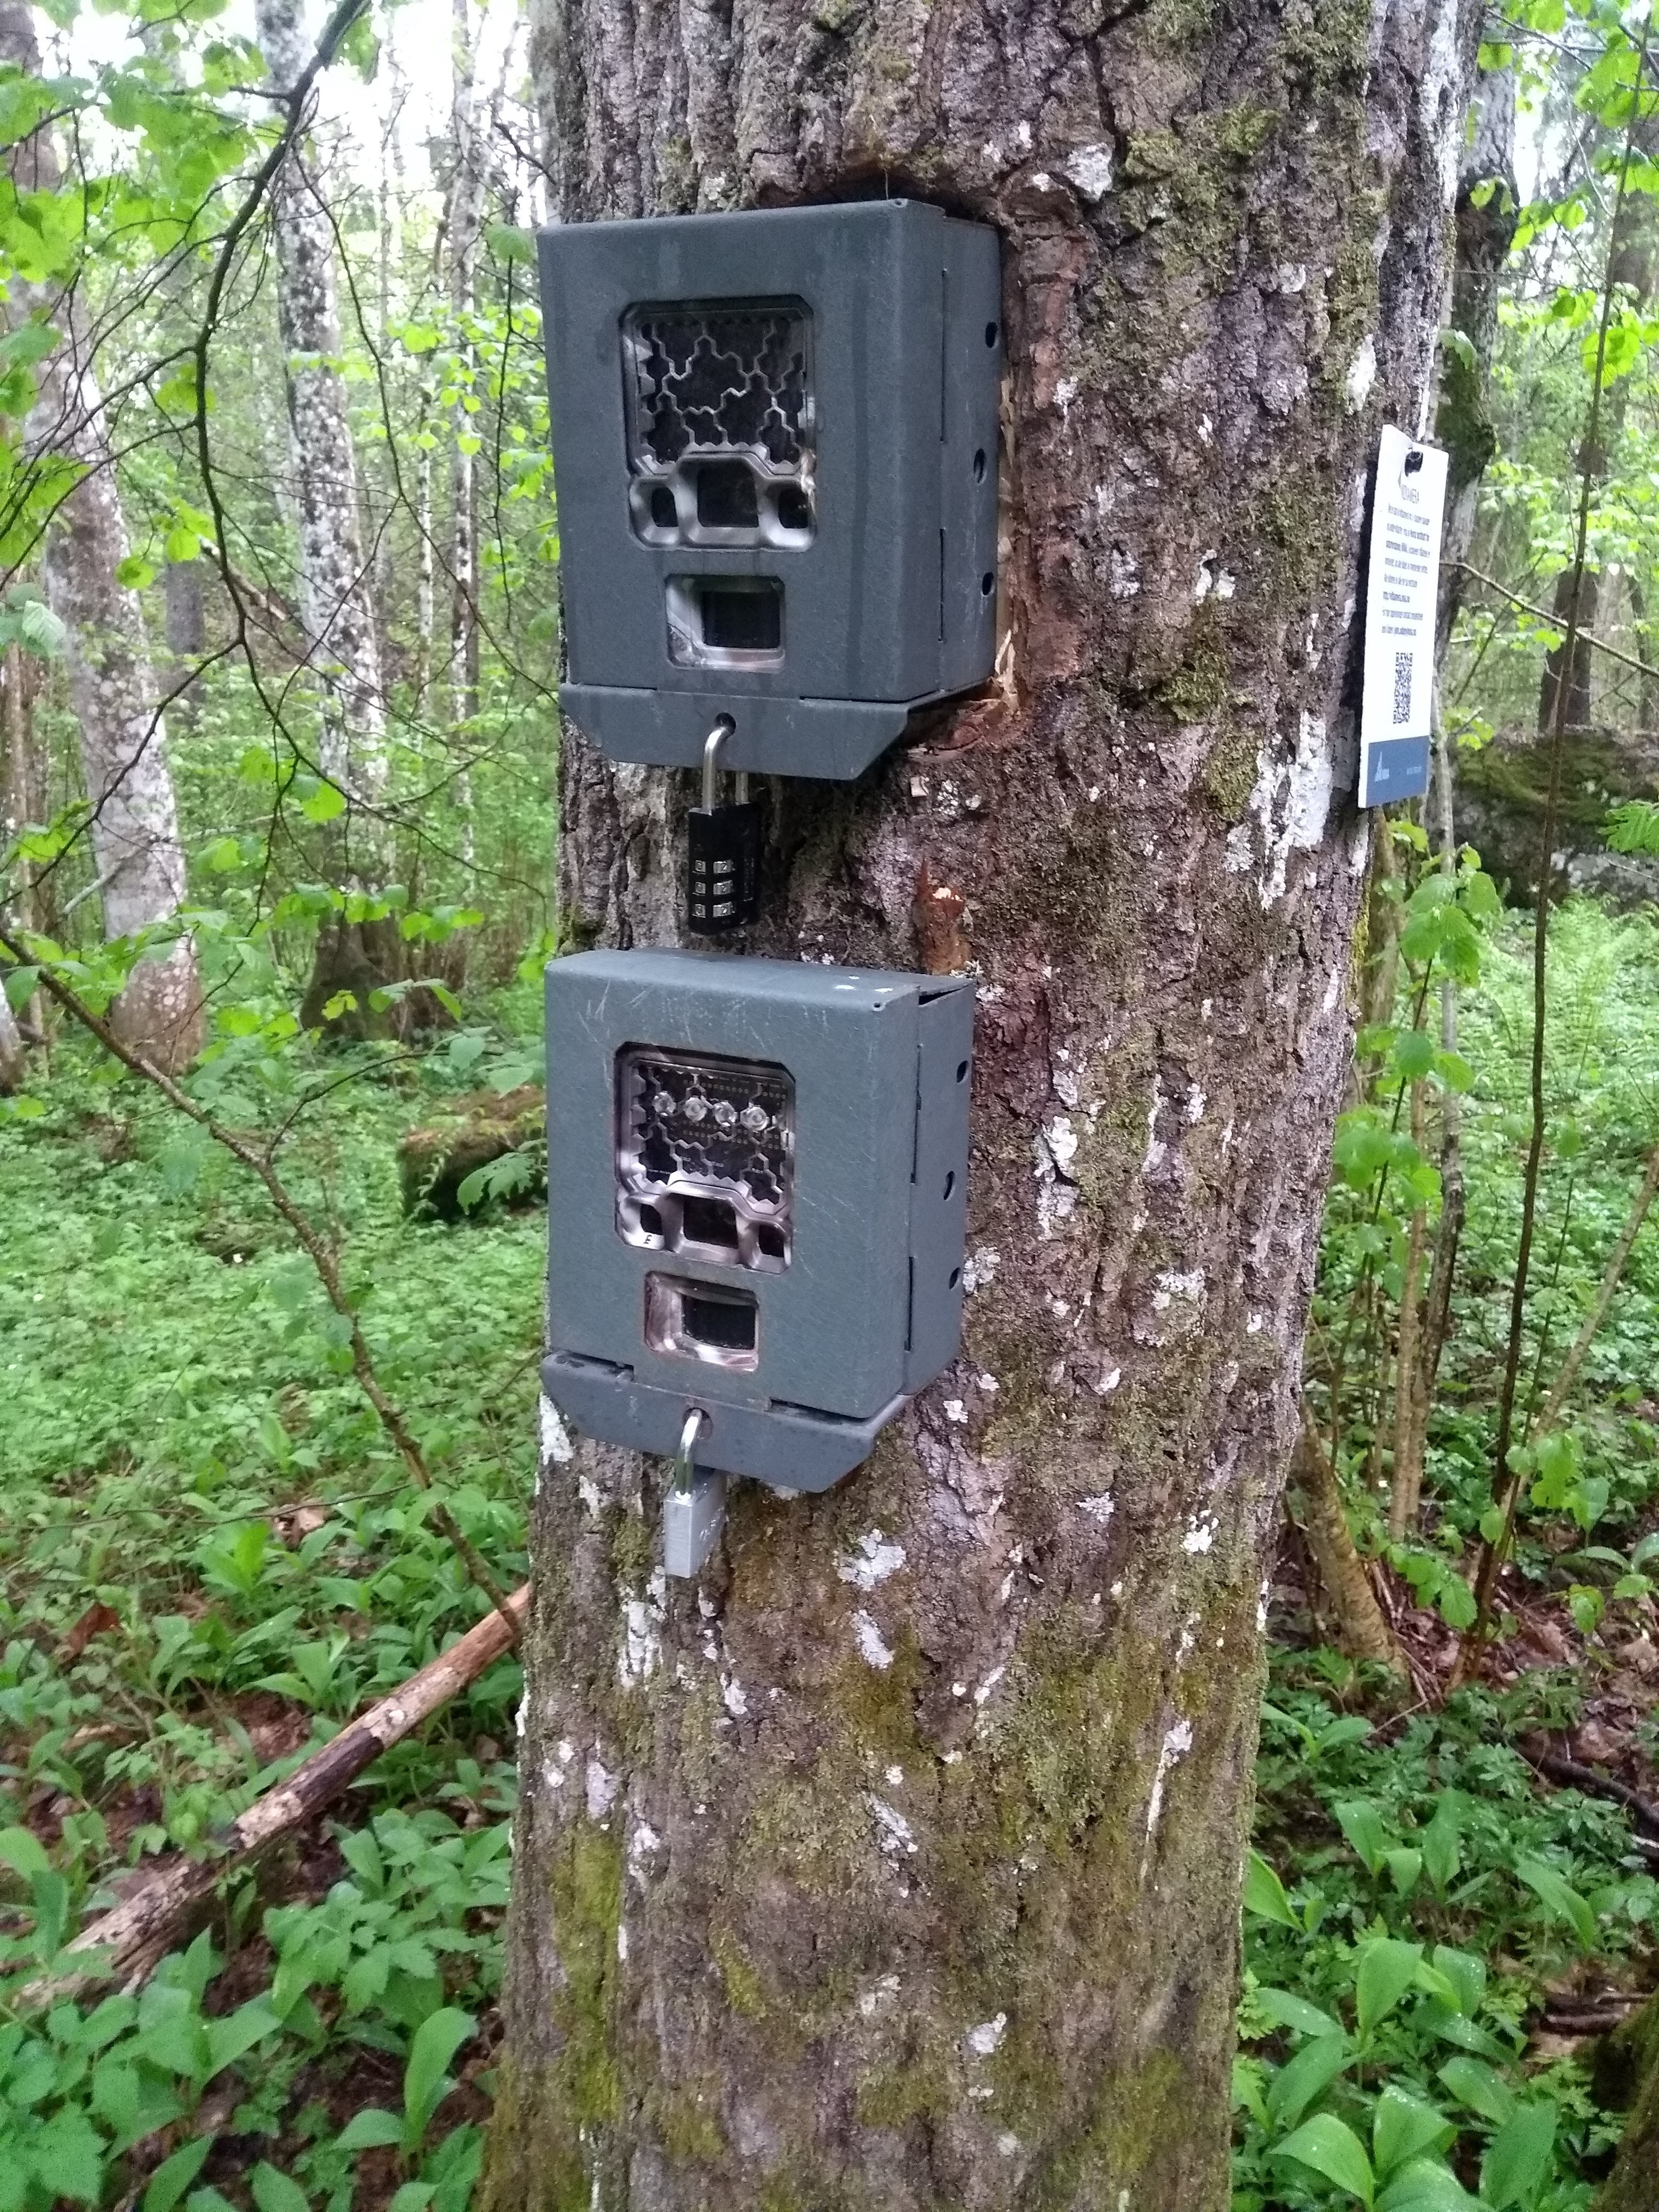
\includegraphics[width=.8\linewidth]{./img/cam_install_example/IMG_20190521_181329313.jpg}
		  \caption{Reconyx IR 160 cm above the ground.\\ Therefore, I positioned the wLED underneath.}
		  	\label{fig:cam_ex_c}
	\end{subfigure}
		\begin{subfigure}{.5\textwidth}
		  \centering
		  	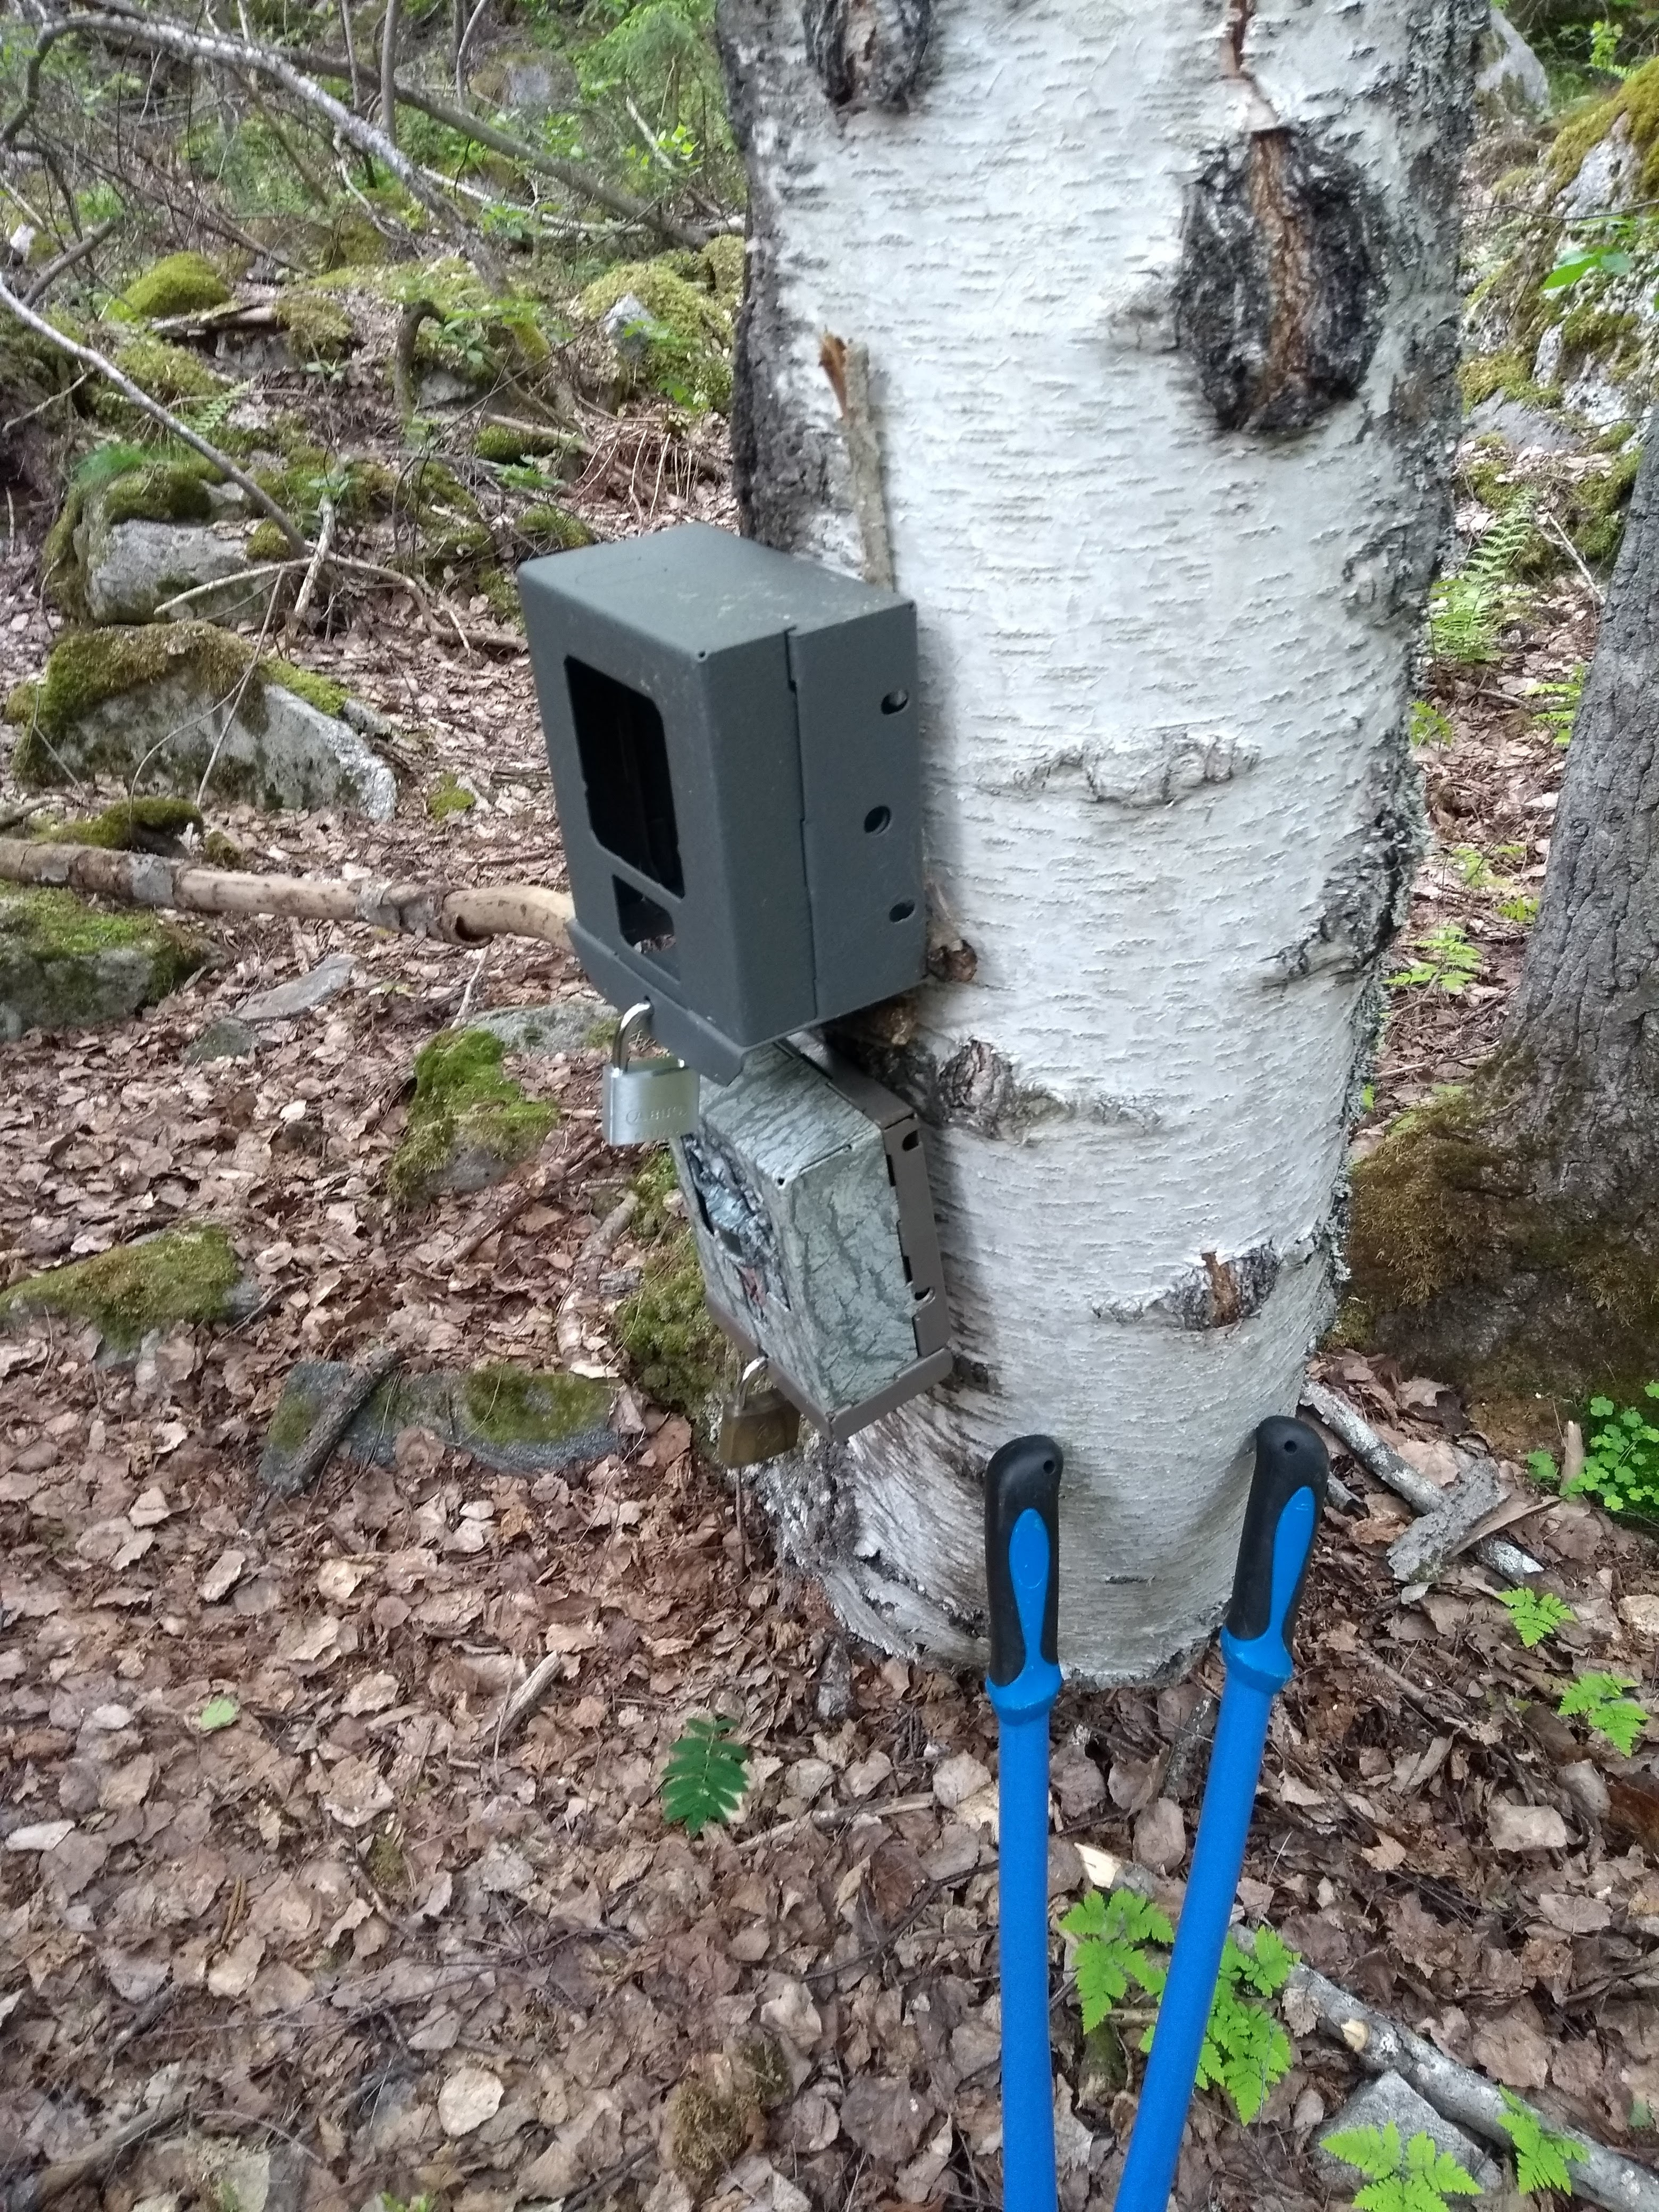
\includegraphics[width=.8\linewidth]{./img/cam_install_example/IMG_20190529_181049340.jpg}
		  \caption{Additional CT boxes remained\\ during IR periods.}
		  	\label{fig:cam_ex_d}
	\end{subfigure}
		\caption[Examples of camera setups]
		{Examples of camera setups %\par \small
		The preinstalled IR cameras varied in the way they were set up. Lower cameras had Infra-Red flash, upper cameras had white LED flash.}
	\label{fig:cam_ex_main}
\end{figure}





I visited sites of the treatment groups at least once every three months in order to move the wLED cameras.
For logistical reasons I visited sites of the control group less often.
However, as the cameras were part of other, ongoing projects, they were occasionally visited by workers from NINA to retreive the Secure Digital memory cards (hereby SD Cards) for data. %write in full on first mention (-Atle)
This was mostly the case for sites close to, and south of, Oslo, or rather, the cameras not normally operated by local volunteers.




%We quantified the degree of consistency in implementing and reporting features of CT protocols and study design that might affect detectability and sampling error (e.g. camera type and settings, spatial and temporal sampling effort, use of attractants; Table S1). These details are fundamental to interpreting results of CT studies and assessing their reliability, repeatability and suitability for broader comparison or synthesis (Meek et al. 2014a)

%TODO Details of camera trap orientation, use of lures, and performance settings are also critical elements of camera trapping methodology. The height in relation to the target, the direction the camera is facing in relation to expected animal travel and path of the sun as well as horizontal and vertical alignment may all influence the results of camera trap studies. Providing clear descriptions of exactly how cameras were placed is fundamental to understanding and interpreting the results of research. (Meek etal 2014)



\section{Data Collection} 




\begin{table}[h]
\caption{Camera models included in the survey}
\label{tab:cam_mod}
\centering

\begin{tabular}{llr}
\hline
Producer  & Model name & Flash type  \\
\hline 
Browning	& Spec Ops: Extreme 					& No-glow IR \\
%\multirow{5}{2cm}{Reconyx HyperFire Series} &
			& HC500 Semi-Covert IR					& Red-glow IR \\
Reconyx		& HC600 High-Output Covert IR			& No-glow IR  \\
HyperFire 	& PC800 Professional Semi-Covert IR 	& Red-glow IR \\
Series 		& PC900 Professional Covert IR 			& No-glow IR  \\
    		& PC850 Professional White Flash LED	& White LED  \\
\hline
\end{tabular}
\end{table}


\begin{table}[h]
\caption[Camera settings and features]
{Camera settings and features %\par \small 
All Reconyx-models were part of the HyperFire series and practically identical in all aspects except for type of flash. Camera specifications are gathered from product reviews (www.trailcampro.com).}
\label{tab:cam_set}
\centering
\begin{tabular}{lcc}
\hline 
 & Browning & Reconyx \\ 
\hline 
Number of cameras 	& 34(?) 	& 26(?) \\  
Trigger speed 		& 0.43 s 	& 0.28 s \\ 
Recovery speed 		& 0.8 s 	& 0.9 s \\ 
Photos per trigger 	& 8 		& 3 \\  
Detection angle 	& 45.5$^{\circ}$ 	& 42$^{\circ}$ \\ 
Field of view 		& 40.6$^{\circ}$ 	& 42$^{\circ}$ \\  
Quiet period 		& No delay 	& No delay \\ 
Trigger interval	& Rapid fire & Rapid fire \\
Time lapse			& No	 	& Yes \\
\hline 
\end{tabular} 
\end{table}



%( CT model and settings (quiet period, SENSOR SENSITIVITY, trigger speed, photograph, burst of photographs or video, type of flash, etc.) ) %TODO add into cam_mod table





As seen in figure \ref{fig:map}, %TODO insert map with loc, white point inside flash-cameras.
there was a correlation between latitude and camera type.

% difference between the two camera types*** 
% Assumptions: chance of detection & sp validation BROWNING > RECONYX, operational days BROWNING < RECONYX


\begin{figure}
	\label{fig:map}
\end{figure}

%* Number and spacing of CTs |Hofmeester 2017 
%Mention in map figure text


%* Temperature and weather during the survey 
%Don't have that data as far as I know





\section{Data processing} %TODO
All SD cards were delivered to NINA for data processing.
Firstly, a facial recognition algorithm (FRA) was used to sort all the pictures. %artificial intelligence software (AI)
Afterwards, a human sorter checks the softwares' output, confirming all the correct decisions (i.e. species detections) and correcting all the wrong ones. 
Consequently, the rate of correctly identified species has gone up as the FRA sometimes detect animals that aren't easily noticed by human sorters (pers.comm. John Odden). 
NINA's goal is to fully automate this identification process, which is a request from The Norwegian Data Protection Authority in relation to usage of cameras in densely crowded areas (e.g. parks) (pers.comm. John Odden).

%Nei, vi har ikke publisert artikkel på gjenkjenningsalgoritmen. Du har jo vært med på prosessen sjøl, så jeg veit ikke om du egentlig trenger referanse her, men du kan sette inn John O som pers med og merke det, så kan han eller jeg endre det slik vi mener det bør være når vi leser gjennom oppgava di..
The wLED CTs were considered as external flashes, and so, only the pictures from the preinstalled IR CTs were sorted for species identification.
NINA provided me with a data frame containing time stamps for every triggering of each IR CT, including all meta data from the CTs, coupled with predicted species (FRA output, with a confidence number), verified species (by human sorters), number of animals and distance from camera.

Thus, if a moose ruminated in front of a camera for 30 minutes, the data frame would include several detections in sequence.
In order to remove autocorrelation in the observations, I defined an event to be any sighting of a species that occured more than 20 minutes after the previous sighting of the same species.
Number of individuals was not taken into account.
My predictor variable of interest was the three different types of periods, namely IR, wLED and Control periods.

I extracted metadata from all pictures taken by the wLED CTs and used that to define the duration of each wLED period.
If a wLED CT stopped working (eg. due to full SD card or empty batteries) before the day I came to move it, the site would have already entered its next IR period.
This happened a few times, which can be seen as the times a light blue period starts outside of the shaded areas in figure \ref{fig:timeseries}.
If an IR CT stopped working during a wLED period, that period represented a GAP even though the wLED CT still functioned. Thus, the site, and it's inhabitant animals, would still experience the effect of a white flash up until the start of the IR period.
I never experienced that both the IR and the wLED CTs of a site had stopped working at the same time.

When modelling the detection rates I needed periods of similar lengths to each other. Therefore, I divided the control group-cameras into four periods of similar lengths to that of the IR- and wLED-periods (see figure \ref{fig:timeseries}). 
%Describing in brief how coding is undertaken is useful for readers to understand the methods used in relation to the results.(Meek etal 2014)


In total, 4 sites were removed before the analysis due to technical faults, or alike.
1 CT was removed from the control group, as it turned out to be a white LED camera.
3 CTs were removed from the treatment groups, because of large or frequent gaps due to technical errors, and at one site, ineffective placement of the additional white LED camera. 



\begin{figure}
		\centering
		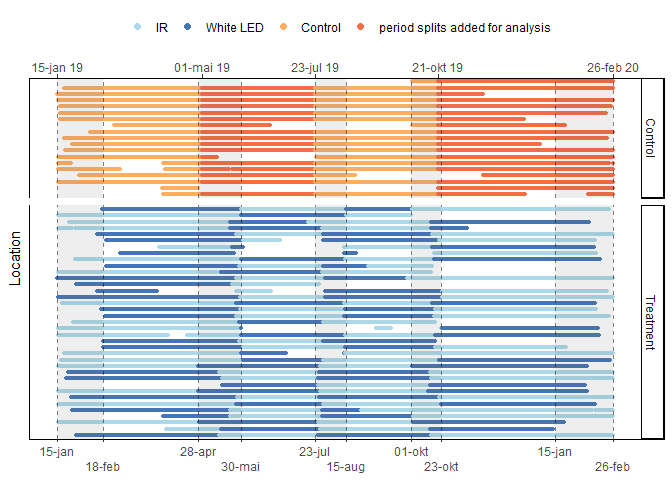
\includegraphics[scale=.8]{../R/FLM_notebook_files/figure-gfm/effort-facet-1.png}	
\caption[Active camera days]
{Active camera days \par \small 
Colours indicate the different periods for each site. White spaces indicate gaps where the IR CTs were inactive. Control camera periods were defined in similar lengths to that of the treatment group during analysis. As a result, the first day of control periods are often set at dates far from when I actually visited the site. Shaded areas represent my field work periods. \label{fig:timeseries}}
\end{figure}


%*************************************************************
%Hypothesis 1: Usage of white LED flash will stress one or more species in general, and therefore lower the detection rate of the stressed species. The effect will likely vary in extent between species.


\section{Statistical analysis} %This is a reference to the session info appendix \ref{app:sessinfo}

To test for effects of the white LED flash I used the R programming language (\cite{RCoreTeam2020}), in the RStudio IDE (\cite{RStudioTeam2020a}), adopting large parts of the tidyverse (\cite{tidyverse}) and the easystats (\cite{easystats}) frameworks along the way. Complete citation of R packages used are presented in appendix \ref{app:sessinfo}. 
%TODO easystats referanse


	\subsection*{GLMM}
To test H1 I looked for differences in detection rate per day, using Generalised Linear Mixed Models (GLMM) with the glmer function from the R package lme4 (\cite{lme4}).
I fitted separate models for each species to avoid overly complicated models. 
Locations that had 0 observations of the modelled species were filtered out before the modelling, but for all locations that had observed the species, all periods were included.
The dependent variable was count data (number of observations), and I therefore assumed the error term followed a Poisson distribution ($ X \sim Pois(\lambda) $).

I included location ID and week of the year as random effects to account for consistent differences between camera sites and seasonal changes during the year of study.
95\% Confidence Intervals (CIs) and p-values were computed using the Wald approximation.
I used standardized parameters (mean = 0, SD = 1) to enable comparison of effect sizes.

The main term of interest was time since deployment interacting with type of flash period (formula: n.obs $\sim$ time.deploy $\ast$ flash).
For the sites that were equipped with an additional white LED camera, time since deployment starts from the day I visited the camera, and set up/ took down the white LED.
The control group’s “day 0” of time since deployment were set at points reflecting the onset of field work each time, in order to obtain periods of similar lengths to that of the white LED-locations.

I trimmed the period lengths down to a reduced maximum length, based on the median length of the IR and white LED periods, to enhance meaningful comparison.
Thus, any period exceeding the shortest median length, was trimmed down, as visualized in figure \ref{fig:median_period}.
Finally, due to large eigenvalues in the fixed effects, the model failed to converge, and an error message prompted me to rescale variables.
Therefore I divided the time since deployment-variable by ten, which solved the error. Consequently, the time axis is shown in days/10, which means that 8 corresponds to 80 days.


\begin{figure}
	\centering
	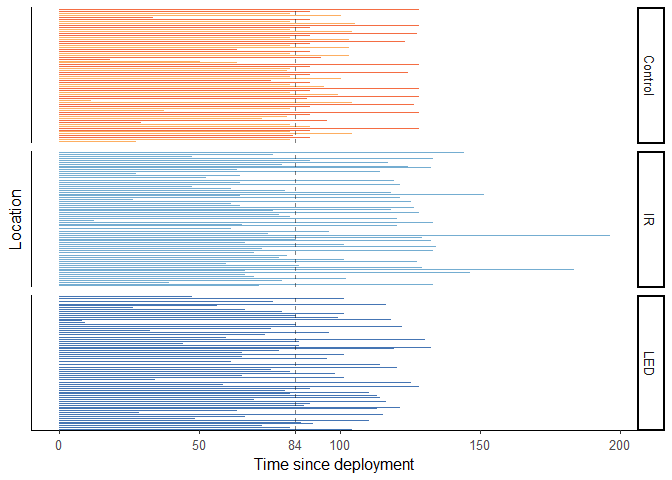
\includegraphics[scale=.8]{../R/glmm_sp_files/figure-html/period-length-wControl-1.png}
	\caption[Period lengths]
	{Period lengths \par \small 
	Vertical line represents the median IR period length, which was shorter than the median of the other groups. Data superceding the median were trimmed away for the GLMM. \label{fig:median_period}}
\end{figure}

%AMkomm: til analyse
If there were any effect of the white LED, the IR period should show a regression to the norm, ie. counteracting the trend during the wLED periods. Thus, if the wLED had a negative slope along the time axis, the IR should have a positive slope.
Further, the detection rate at the start of each period, should correspond somewhat to the detection rate at the end of the previous period. Still, that pattern could be skewed to some extent due to my visitation of each location at the start of all IR and wLED periods.






\subsection*{Equivalence test}
% Multiple testing i arkiv/method-ark
I used the standard significance level of $\alpha = .05$, and performed an equivalence test on my model outputs, using the function equivalence\_test from the R package parameters ().%\cite{package-parameters}). %TODO
In an equivalence test, model parameters are tested against a Region of Practical Equivalence (ROPE) as opposed to merely one single mean value, thus accounting for the \emph{effect size} of each parameter.
If the parameters estimate and CI falls outside the ROPE, their null hypothesis is rejected. However, if the CI is inside the ROPE, H0 is accepted, no matter if a standard Null Hypothesis Significance Test (NHST) would have deemed it significant.

Inside the function equivalence\_test I used the Two One-Sided Tests (TOST) rule, where the confidence interval (CI) is set to $1 - 2\times \alpha$. In my case that gave a narrow CI of 0.90.
For models from count data, the residual variance is often used to define the ROPE range. However, the description of the rope\_range function from the package bayestestR () states this threshold as "rather experimental" and that the range is probably often similar to the default [-0.1, 0.1] of a standardized parameter (www.easystats.github.io/bayestestR/reference/rope\_range.html, accessed 11.3.2021). %TODO betre ref-metode for nettsider
Hence, I used the default ROPE range which corresponds to a negligible effect size according to Cohen, 1988.

%In the TOST procedure, the null hypothesis is the presence of a true effect of DL or DU, and the alternative hypothesis is an effect that falls within the equivalence bounds or the absence of an effect that is worthwhile to examine. \cite{Lakens2017}










